\chapter{Physics at the ILC}

  In the chapter \ref{chap:SM}, the framework of particles physics was described. 
  Since the beginning of High Energy Physics, different experiments have been done to confirm the exactness of the SM but also to find new physics beyond the SM.
  The beam structure allow different kind of measurements.
  For example, the LHC has a high luminosity and high energy beam, able to reach new energy scale on earth, whereas the ILC is trying to reach more precise results, with less energy.
  This chapter will discuss the physics that will be studied at the ILC.
  It will focus particularly on the Higgs physics.
  An introduction to a physic analysis will be given. 
 
 \minitoc

  \section{Potential studies}

  As seen in chapter \ref{chap:ILC}, the ILC will have a vast and variable tunable centre-of-mass energy.
  Due to the features of an $e^+e^-$ collider, the initial state of collision is well defined.
  Contrary to the LHC, there are no strong interaction backgrounds and the electroweak background is controlled and calculable.
  This conditions will help to perform precise measurements and looking for new physics. 
  
  For example, the ILC will be able to collect more Z boson events than the LEP did at the centre-of-mass energy $\sqrt{2} = 91$ GeV.
  It will allow to perform ultra precise measurements of the Z boson and the electroweak sector to study the Z asymmetries and couplings, but also to measure rare processes that where limited by statistics at LEP.
  
  By increasing the centre-of-mass energy to $\sqrt{s} = 160$ GeV, ultra precise measurements of the W mass could be performed (MeV precision) and with higher energy, it is also possible to measure precisely the W boson couplings.
  Also, at higher energy, there is a new perspective to measure precisely the nature of the Higgs boson and its coupling.
  The large statistics given by the ILC will permit to study rare Higgs decay.

  Top physics

  New physics
  

  \begin{table}[h]
    \begin{center}
    \begin{tabular}{c c c}
      \hline %----------------------------
      Energy (GeV) &  Reaction  &  Physics Goal \tabularnewline
      \hline %----------------------------
      \hline %----------------------------
      91  &  $e^+e^- \rightarrow Z $ & ultra-precision electroweak \tabularnewline
      \hline %----------------------------
      160 & $e^+e^- \rightarrow WW $ & ultra-precision W mass \tabularnewline
      \hline %----------------------------
      250 & $e^+e^- \rightarrow Zh$ & precision Higgs coupling \tabularnewline
      \hline %---------------------------- 
      \multirow{3}*{350 - 400} & $e^+e^- \rightarrow t\overline{t}$ & top quark mass and couplings \tabularnewline
                               & $e^+e^- \rightarrow WW $ & precision W couplings \tabularnewline
                               & $e^+e^- \rightarrow \nu\overline{\nu}h$ & precision Higgs couplings\tabularnewline
      \hline %----------------------------
      \multirow{5}*{500} & $e^+e^- \rightarrow f\overline{f}$ & precision search for Z' \tabularnewline
                         & $e^+e^- \rightarrow t\overline{t}h $ & Higgs coupling to top \tabularnewline
                         & $e^+e^- \rightarrow Zhh $ & Higgs self-coupling \tabularnewline
                         & $e^+e^- \rightarrow \tilde{\chi}\tilde{\chi} $ & search for supersymmetry  \tabularnewline
                         & $e^+e^- \rightarrow AH, H^+ H^-$ & search for extended Higgs states \tabularnewline
      \hline %----------------------------
      \multirow{4}*{700-1000} & $e^+e^- \rightarrow \nu\overline{\nu}hh$ & Higgs self-coupling\tabularnewline
                              & $e^+e^- \rightarrow \nu\overline{\nu}VV$ & composite Higgs sector\tabularnewline
                              & $e^+e^- \rightarrow \nu\overline{\nu}t\overline{t}$ & composite Higgs and top\tabularnewline
                              & $e^+e^- \rightarrow \overline{t}\overline{t}^*$ & search for supersymmetry\tabularnewline
      \hline %----------------------------
    \end{tabular}
    \end{center}
      \caption{Summary of the major processes that will be studied at the ILC for different energies\cite{Baer2013}.}
      \label{taf:physicsAtIlc}
  \end{table}
  
  \section{Higgs physics}

  \subsection{Production of the Higgs at the ILC}

  Contrary to the LHC, the Higgs will be accessible by direct measurement. 
  They are three major processes Higgs boson production at the ILC, the Higgs-strahlung, the WW-fusion and the ZZ-fusion:

  \begin{description}
    \centering
    \item[Higgs-strahlung:] $e^+e^- \rightarrow ZH \rightarrow f\overline{f}X$
    \item[WW-fusion:] $e^+e^- \rightarrow \nu \overline{\nu} W^+W^- \rightarrow \nu \overline{\nu} H$
    \item[ZZ-fusion:] $e^+e^- \rightarrow e^+e^- ZZ \rightarrow e^+e^- H$
  \end{description}

  The Higgs-strahlung is a s-channel process that is dominant at 250 GeV and its cross-section falls off as 1/s as the centre-of-mass energy $\sqrt{s}$ increases.
  The WW-fusion and ZZ-fusion are t-channel processes. 
  The cross-section grows logarithmically with the center-of-mass energy and the contribution of the fusion processes is small at 250 GeV.

  The polarisation of the beam will help the experimenters to select Higgs reactions or to change the mixture of signal and background.
  For example, the WW-fusion occurs only with left-handed electrons associated to right-handed positrons. 


  \begin{figure}{h}
    \centering
    \missingfigure{Feynman diagrams of Higgs production}
    \caption{The higgs production processes at the ILC.}
    \label{fig:higgsProd}
  \end{figure}

  The figure \todo{ADD REF TO THE FIGURE} shows the cross-section production of the Higgs at the ILC regard to the energy of the collision.
  
  \begin{figure}
    \centering
    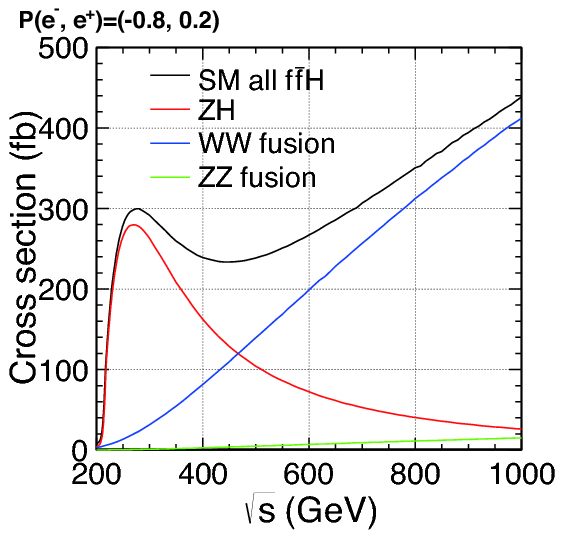
\includegraphics[width = 10 cm]{Pictures/Higgs/higgs_xsec_P-8_3.png}
    \caption{The cross section production of the Higgs boson with a mass of 125 GeV. REF HIGGS WHITE PAPER}
    \label{fig:higgsXsec}
  \end{figure}

  \subsection{Decays of the Higgs}

  The Higgs boson couples to all the particles of the SM.
  There are many decay modes: $b\overline{b}$, $WW$, $ZZ$, $gg$, $c\overline{c}$, $\tau \tau$, $\gamma \gamma$, $\gamma Z$
  At the LHC, the decay $h \rightarrow b\overline{b}$ can be observed with special kinematics but the $h \rightarrow c \overline{c}$ and $h \rightarrow gg$ decays are extremely challenging to observe.


  \section{Advantages of the ILC}

  The \gls{ILC} has the main advantage to produce events non accessible at the \gls{LHC}.
  Through this section, some benefits of the \gls{ILC} are introduced thanks to a simple analysis of simulated data at 350 GeV.
  
  The goal of this section is to present how to perform an analysis from simulated data. 
  Measuring the Higgs coupling to $c\overline{c}$ is important to have a reference value to understand any deviations form the SM predictions in the Higgs coupling to $t\overline{t}$ and $gg$.
  To study this coupling, the analysis will be focus on the final state that gives two neutrinos and two jets coming from the Higgs.
  
  \subsection{Background processes}

  They are many background to take into account:    
